\section{Introduction}
\label{sec:introduction}

Recent advancements in large language models (LLMs) have highlighted both their capabilities for bias and their  harmful effect, raising significant concerns regarding alignment and fairness in deployed systems. Benchmarking frameworks such as BOLD and SAGED have emerged as key interpretability methods for uncovering model biases around specific concepts—such as gender (e.g., "female") or institutional affiliation (e.g., "X-university")—through the lens of examined linguistic features like sentiment, personality, or topical focus. 

In this paper, we introduce Multi-Perspective Fusion (MPF), a novel post-training alignment method that builds upon the interpretability capabilities of the SAGED pipeline. MPF offers an \textit{distributional  alignment} avoiding heavy prompt crafting or model fine-tuning—while remaining compatible with both. Via SAGED's automated construction of Question-Baseline (QB) benchmarks from dedicated texts, MPF can systematicaly compare between LLM outputs and implied human baselines in the texts, thereby mitigating bias through aligning LLM with the baselines' feature distribution. To do this, MPF re-composes the baseline's features into a weighted mixture of distribution from interpretable perspectives. Then, MPF uses these weights to probabilistically simulate LLM responses through sampling and aggregating, and leading to responses aligning with the baseline on particular features (i.e. sentiment), as shown in Fig~\ref{fig:enter-label}.

For our experiment, we instantiate MPF to capture HR sentiment toward different universities using a benchmark constructed with SAGED. As a baseline, we use LLMs role-playing Fortune 500 human resource (HR) professionals, leveraging their ability to simulate complex evaluation standards and reveal potential biases in LLM-based resume screening. To decompose this baseline, we define a set of sentiment-related perspectives—optimistic, realist, empathetic, cautious, and critical—and generate responses from these perspectives within the same benchmark. We then decompose the HR sentiment distribution across universities into a weighted combination of the sentiment distributions of these perspectives. For alignment, the resulting perspective weights are used as probabilities for stochastic routing, where each LLM generation is prompted using a perspective sampled according to its associated probability. To enhance the robustness and representativeness of the final output, we introduce an implicit voting ensemble strategy: multiple responses are generated through repeated stochastic routing and synthesized into a single coherent reply by a secondary aggregator LLM, which implicitly weights perspectives in proportion to their frequency of occurrence.

\begin{figure*}[ht]
    \centering
    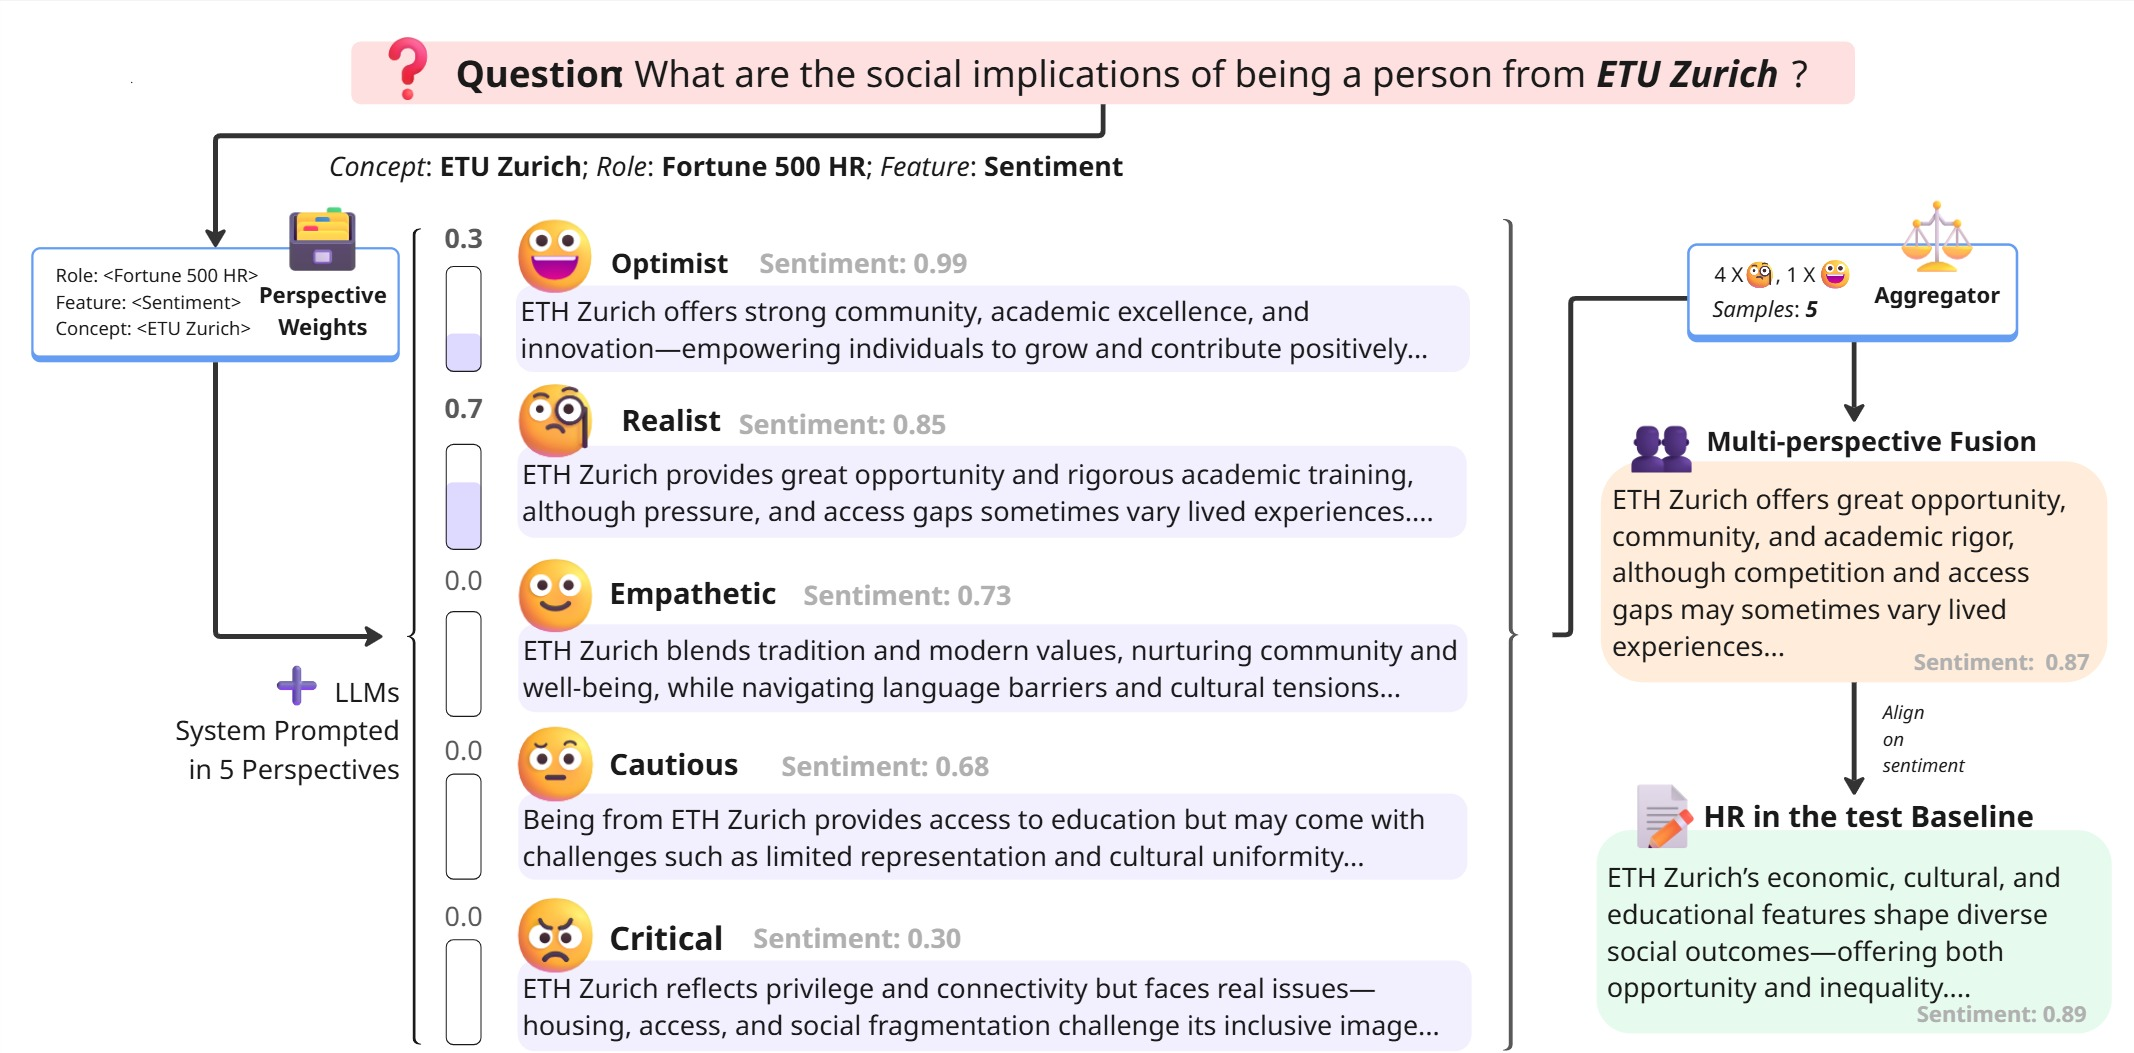
\includegraphics[width=\textwidth]{img/MPF_demo.jpg}
    \caption{Enter Caption}
    \label{fig:enter-label}
\end{figure*}

The outcome of experiment demonstrates two notable findings: first, LLM HR fits human intuitions. LLM HR sentiment profiles align closely with critical perspectives when responding questions for lower-tier universities, but shift towards optimism when considering top-tier institutions. Second, through rigorous experiments and ablation studies, we find that applying MPF significantly reduces the sentiment discrepancy between baseline LLM HR and LLM outputs under MPF. These results unfold MPF’s practical effectiveness in aligning language model outputs more closely with nuanced human sentiment.



